\documentclass{article}
\usepackage{preamble}

\title{Unit 11: Terrestrial Planets}
\author{Astronomy\footnote{Access for free at \href{\openstax}{\openstax}} \hspace{0.1ex} at Cypress Springs High School}
\date{Updated on \today}

\numberwithin{equation}{section}
\setcounter{section}{11}
\numberwithin{figure}{section}

\usepackage{fancyhdr}
\pagestyle{fancy}
\renewcommand{\headrulewidth}{0pt}
\renewcommand{\headruleskip}{0mm}
\fancyfoot[C]{Access for free at \href{\openstax}{\openstax} \hfill \thepage}
\fancyhead{}

% \makenoidxglossaries

\begin{document}

\maketitle

\subsection{Introduction}

\def\aMer{0.387}
\def\aVen{0.723}
\def\aEar{1}
\def\aMar{1.52}
\def\aAB{2.7} %Asteroid Belt peak
\def\aJup{5.20}
\def\aSat{9.57}
\def\aUra{19.17}
\def\aNep{30.18}

\begin{center}
    \begin{tikzpicture}
        \begin{axis}[
            width=\textwidth,
            clip=true,
            axis equal image=true,
            xmin=-0.15,xmax=1.05*\aJup,
            ymin=-\aMar,ymax=\aMar,
            axis line style={draw=none},
            ticks=none,
            cycle list={
                only marks,mark=*,fill=lightgray,draw=black,mark size=0.5pt\\
                only marks,mark=*,fill=lightgray,draw=black,mark size=0.5pt\\
              },
            domain=360-45:360+45,
            samples=1000,
        ]
            \draw[thick,black,fill=yellow] (0,0) node[right=2.5mm] {$\Sun$} 
            circle (0.1);
            \draw (0,0) circle (\aMer);
            \draw[fill=black] (\aMer,0) circle (2pt) node[right=1pt] {$\Mercury$};
            \draw (0,0) circle (\aVen);
            \draw[fill=black] (\aVen,0) circle (2pt) node[right=1pt] {$\Venus$};
            \draw (0,0) circle (\aEar);
            \draw[fill=black] (\aEar,0) circle (2pt) node[right=1pt] {$\Earth$};
            \draw (0,0) circle (\aMar);
            \draw[fill=black] (\aMar,0) circle (2pt) node[right=1pt] {$\Mars$};
            \draw[dashed, gray] (0,0) circle (\aJup);
            \draw[fill=gray] (\aJup,0) circle (2pt) node[right=1pt] {$\Jupiter$};
            \addplot ({(\aAB+0.8*rand)*cos(x)},{(\aAB+0.8*rand)*sin(x)});
            \node[right] at (3.5,0) {Asteroid Belt};
            \draw (3.5,1.45) -- ++(axis direction cs: 1,0) node[right] {\SI{1}{AU}};
            
        \end{axis}
    \end{tikzpicture}
    \captionsetup{type=figure,margin=1in}
    \captionof{figure}{The Sun ($\Sun$) and the terrestrial (inner) planets: Mercury ($\Mercury$), Venus ($\Venus$), Earth ($\Earth$), and Mars ($\Mars$), and the surrounding asteroid belt. The spacing between the planets is to scale, with \SI{1}{AU} being the distance from Sun to Earth. Planetary sizes are not to scale. While Jupiter ($\Jupiter$) is not a terrestrial planet, it is shown here to show the scale and spacing between the inner and outer planets.}
\end{center}

\subsection{Mercury ($\Mercury$)} \label{IF2QAz}

Mercury is the closest planet to the Sun and is named after the Roman messenger of the gods. It takes 88 days to complete one orbit around the Sun, traveling at an orbital speed of over 100,000 miles per hour. Its semi-major axis---which is loosely defined as its average distance to the Sun---is \SI{0.39}{AU}, or 58 million km. (Recall that, by comparison, Earth is at \SI{1}{AU}.) Because it's so close to the Sun, Mercury is difficult to detect as it never rises high in the sky and it disappears below the horizon shortly after sunset. Moreover, it's similar to the Moon in at least two ways: it lacks an atmosphere and it's heavily cratered. 

\vspace{1em}

Mercury is the smallest terrestrial planet, having a diameter of 4878 kilometers, which is only a few hundred miles more than the distance from Seattle, Washington to Miami, Florida. Its interesting composition makes it unique among the planets. Mercury's high density (\SI{5.4}{g/cm^3}), which is higher than Earth's Moon, implies that the planet is made mostly of heavier materials such as metals. Computer and mathematical models suggest that 60\% of its total mass comes from a metallic core made of iron and nickel. The rest of the planet is made up primarily of silicates. As the core's diameter is 3500 kilometers, you could think of Mercury as a metal ball the size of the Moon surrounded by a rocky crust 700 kilometers thick. Mercury has a weak magnetic field, so at least part of the core must be liquid in order to generate this observed field.

\vspace{1em} 

For many years, it was widely believed that Mercury does not rotate but keeps one face to the Sun. An implication of this belief is that one side is perpetually hot while the other is always cold. Radar observations of Mercury in the mid-1960s demolished those beliefs and proved that Mercury rotates.  This discovery was proved by measuring something called the Doppler radar shift. When a planet is turning, one side of the planet is moving towards Earth while the other is moving away. Scientists who aim to measure the rotation transmit electromagnetic radar waves at a precise frequency towards the planet. The incoming waves strike the planet's surface and reflect back to Earth to be analyzed. If the receiving planet is not rotating, all waves that reflect off the surface will arrive back to Earth at the \textit{same} frequency as the originally transmitted waves. But if the planet \textit{is} rotating, the side rotating towards Earth reflects a wave with a frequency that is higher than the frequency of the transmitted wave. Conversely, the side rotating away from Earth reflects a lower-frequency wave. Therefore, the reflected waves that are received back on Earth will not arrive at a single frequency but at a \textit{range} of frequencies. This spreading of frequencies is known as \textit{broadening}. Broadening is direct evidence of planetary rotation. The degree of broadening provides an exact measurement of the rotation rate of the planet. Thus it was measured that Mercury orbits once on its axis every 59 days. In other words, one day on Mercury lasts 59 Earth-days! See the \texttt{Day on Mercury} simulation for a visual comparison of the Mercurian day and year [\href{https://sciencesims.com/sims/mercury-orbit/}{click here}].

\begin{center}
    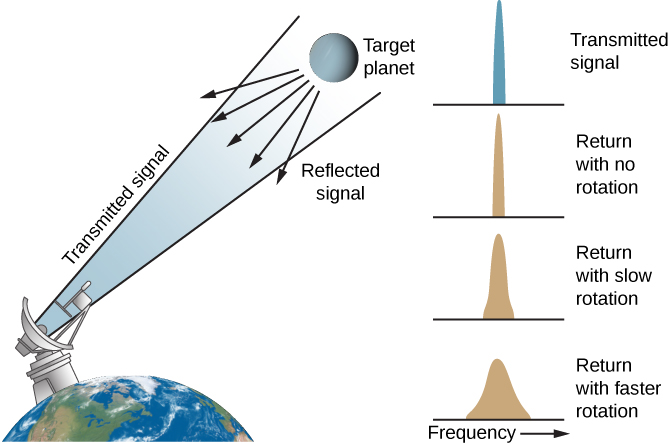
\includegraphics[width=9cm]{Figures/Figure9.21.jpeg}
    \captionsetup{type=figure,margin=1in}
    \captionof{figure}{The Doppler radar shift and frequency broadening used to measure planetary rotation.}
\end{center}


\subsection*{\ref{IF2QAz} Exercises}

\begin{exercise}
    List 2 similarities between Mercury and the Moon, and 2 differences.
\end{exercise}

\begin{exercise}
    True or False? Mercury lacks a magnetic field.
\end{exercise}

\begin{exercise}
The fraction of a day to a year on Earth is 1/365. Express the day-to-year ratio on Mercury as a simplified fraction.  To arrive at a true simple fraction, you may approximate the ratio.
\end{exercise}

\begin{exercise}
    What is the interesting size-comparison between the Moon and Mercury's crust and interior?
\end{exercise}

\begin{exercise}
    Summarize the composition of Mercury.
\end{exercise}

\begin{exercise}
    In your own words, explain how scientists in the 60s proved that Mercury rotates once every 59 days.
\end{exercise}

\begin{exercise}
    What is the distance from the Sun to Mercury, in astronomical units, kilometers, and miles?
\end{exercise}

\begin{exercise}
    Where does the name ``Mercury'' come from?
\end{exercise}

\clearpage

% \begin{mdframed}[backgroundcolor=black!10]
%     The character Mercury, the Roman messenger of the gods, originated in his Greek counterpart named Hermes. Thus many of the stories related to Hermes were also attributed to Mercury. One such story goes as follows.

%     \vspace{1em}

%     Hermes was born in a cave in Kyllene. He was the son of Zeus and Maia, who was one of the Pleiades (the seven sisters, or daughters of Atlas). One day, while Hermes was still a baby, wrapped in swaddling clothes and sheltered in his cradle, he sneaked out of his cradle, put on a pair of boots to cover his tracks, and travelled toward Pieria, where he stole cattle belonging to the god Apollo. He led the cattle to Pylos. During his journey, he sacrificed two cows, while cooking some of the meat, and hid the rest in a small cave. 

%     \vspace{1em}

%     Hermes encountered a tortoise munching on food outside the cave. He picked up the tortoise, cleaned and polished its shell, and used leftover material from the cows he had sacrificed to attach several strings from the edge of the shell. After adding a few more attachments to the shell and applying tension to the strings, he succeeded in inventing the first lyre, a small string instrument which played beautiful music. 

%     \vspace{1em}

%     A furious Apollo, upon discovering that his cattle was missing, went around Pylos in search for the thief. He interviewed the locals, who hinted that a boy was seen traveling with his cattle. 
% \end{mdframed}

% \clearpage

\subsection{Venus ($\Venus$)} \label{oSXifU}

Venus is the second planet from the Sun. Its orbit is very nearly circular, at a distance of 108 million kilometers (\SI{0.72}{AU}) from the Sun. Like Mercury, Venus sometimes appears as an ``evening star'' and sometimes as a ``morning star.'' Venus approaches Earth more closely than does any other planet: at its nearest, it is only 40 million kilometers from us.

\vspace{1em}

Venus appears very bright in the night sky. Viewing it through a telescope telescope reveals that it goes through phases like the Moon. Galileo used these phases of Venus as an argument to show that Venus must circle the Sun and not Earth. The planet's actual surface is not visible because it is shrouded by dense clouds that reflect about 70\% of the sunlight that falls on them. So, even with cameras in orbit near the planet, there's no chance to see the surface.

\begin{center}
\begin{tikzpicture}[scale=0.9, transform shape]
    \clip (0,0) circle (2.3cm);
    \node at (-0.02,0.08) 
        {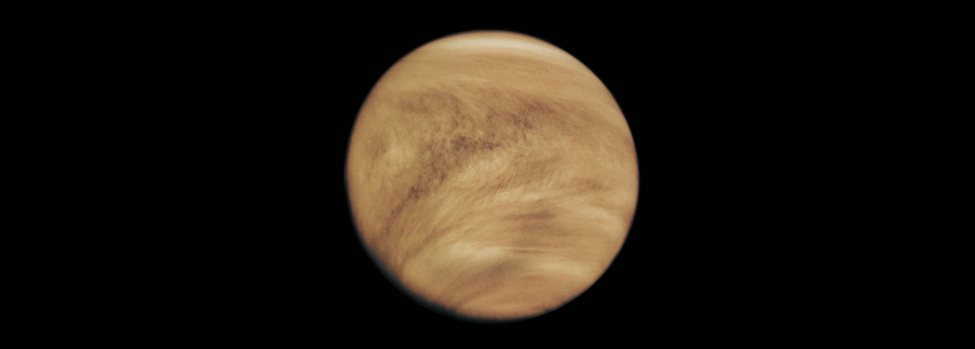
\includegraphics[width=6cm,trim={5cm 2mm 5cm 2mm}, clip]{Figures/Figure10.2.jpeg}};
    \end{tikzpicture}
    \captionsetup{type=figure,margin=1in,font=scriptsize}
    \captionof{figure}{\textbf{Venus as Photographed by the Pioneer Venus Orbiter.} This ultraviolet image shows an upper-atmosphere cloud structure that would be invisible at visible wavelengths. Note that there is not even a glimpse of the planet’s surface. (credit: modification of work by NASA)}
\end{center}

The rotation period of Venus can be found only by bouncing radar signals off the planet, just as in the case for Mercury (see Section \ref{IF2QAz}). The first radar observations of Venus' rotation made in the early 1960s revealed the planet spinning on its axis once every 243 days! Furthermore, these observations revealed another surprise: Venus spins in a backward (or ``retrograde'') direction; that is, from east to west.

\vspace{1em}

Venus orbits the Sun once every 225 days. So the day on Venus (as defined by its spinning once) is longer than the year! Alternatively, if we define 1 day on Venus as the time the Sun takes to return to the same place in Venus' sky, then 1 Venus day is 117 Earth days. Either way, if you say ``See you tomorrow'' on Venus, you’ll have a long time to wait. Although we do not know for sure the reason for Venus' slow backward rotation, it possibly may have suffered one or more extremely powerful collisions during the formation process of the solar system.

\vspace{1em}

The following table compares some basic properties between Earth and Venus.

\begin{center}
\begin{tabular}{|l|c|c|}
\hline
\textbf{Property} & \textbf{Earth} & \textbf{Venus}\\
\hline
Semimajor axis (AU)	& 1.00	& 0.72\\ \hline	
Period (days) & 365 & 225\\	\hline	
Mass (Earth = 1)	& 1.00 &	0.82\\	\hline	
Diameter (km)	& \num{12756} & \num{12102}	\\ \hline	
Density (\SI{}{g/cm^3})	& 5.5	& 5.3 \\\hline	
Surface gravity (Earth = 1)	& 1.00	& 0.91\\	\hline	
Escape velocity (km/s)	& 11.2	& 10.4\\	\hline	
Rotation period & 23.9 hours &	243 days\\	\hline	
Surface area (Earth = 1)	& 1.00 & 0.90\\	\hline	
Atmospheric pressure (bar)	& 1.00 & 90	\\ 
\hline
\end{tabular}
\end{center}

\clearpage

\subsection*{\ref{oSXifU} Exercises}

\begin{exercise}
    Watch ``The First and Only Photos From Venus'' on \texttt{YouTube} (\href{https://youtu.be/M5pXx_AjjlM}{click here}).
\end{exercise}

\begin{exercise}
    What is the distance from Venus to the Sun, in kilometers (km) and in astronomical units (AU)?
\end{exercise}

\begin{exercise}
    Identify a similarity between Venus and our Moon.
\end{exercise}

\begin{exercise}
    Why is it impossible to see the surface of Venus from outside the planet?
\end{exercise}

\begin{exercise}
    How many days does it take Venus to orbit the Sun?
\end{exercise}

\begin{exercise}
    How long does it take Venus to rotate once on its axis?
\end{exercise}

\begin{exercise}
    Identify the unique property related to the direction of Venus' rotation.
\end{exercise}

\begin{exercise}
    How does the air (atmospheric) pressure on Venus compare to that on Earth?
\end{exercise}

\clearpage

\subsection{The Massive Atmosphere of Venus} \label{L8rXjS}

\begin{center}
    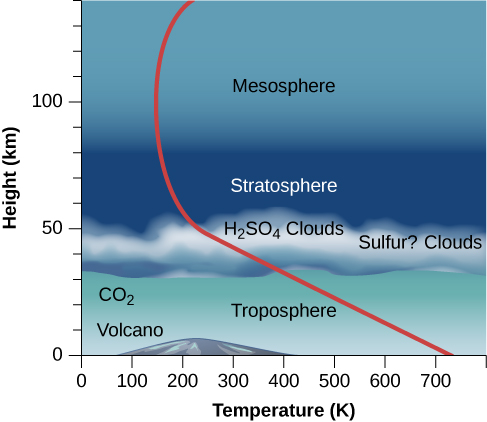
\includegraphics[width=8cm]{Figures/Figure10.12.jpeg}
    \captionsetup{type=figure,margin=1in,font=scriptsize}
    \captionof{figure}{\textbf{Venus' Atmosphere}. The layers of the massive atmosphere of Venus shown here are based on data from the Pioneer and Venera entry probes. Height is measured along the left axis, the bottom scale shows temperature, and the red line allows you to read off the temperature at each height. Notice how steeply the temperature rises below the clouds, thanks to the planet’s huge greenhouse effect.}
\end{center}

\subsection*{\ref{L8rXjS} Exercises}

\textbf{\href{https://openstax.org/books/astronomy-2e/pages/10-3-the-massive-atmosphere-of-venus}{CLICK HERE} to access the text on The Massive Atmosphere of Venus.} 

\begin{exercise}
    Is it generally windy on the surface of Venus?
\end{exercise}

\begin{exercise}
    What is the most abundant gas in the atmosphere of Venus? What percent of the atmosphere does it represent?
\end{exercise}

\begin{exercise}
    The atmospheric pressure at the surface of Venus is extremely large due to its massive atmosphere. How deep below the ocean surface on Earth would you have to be to experience a comparable pressure?
\end{exercise}

\begin{exercise}
    Identify the chemical composition (including the molecular formula) of the clouds that exist about 50 kilometers above the surface.
\end{exercise}

\begin{exercise}
    When was it discovered that Venus is so hot?
\end{exercise}

\begin{exercise}
    The surface temperature on Venus can exceed \SI{700}{K}. Convert this temperature from Kelvin to Fahrenheit using the following formula:

    \begin{equation*}
        T_{\SI{}{\degree F}} = \frac{9}{5} \left(T_{\text{K}} - 273.15 \right) + 32
    \end{equation*}

where $T_{\SI{}{\degree F}}$ is temperature in degrees Fahrenheit, and $T_{\text{K}}$ is temperature in Kelvin.
\end{exercise}

\begin{exercise}
    How many times more carbon dioxide ($\text{CO}_2$) does Venus have in its atmosphere compared to Earth's?
\end{exercise}

\begin{exercise}
    Venus may once have had a climate similar to that of Earth. List some features of this possible climate from Venus' history.
\end{exercise}

\begin{exercise}
    Hydrogen (H) is the first element of the periodic table. With one proton and one electron, it's an extremely light gas at high temperatures. Explain what happens to hydrogen gas in the atmosphere. 
\end{exercise}

\begin{exercise}
    When water is lost from a planet's atmosphere, can it be restored?
\end{exercise}

\clearpage

\subsection{Mars ($\Mars$)} \label{3uBag7}

Mars is the fourth planet from the Sun. The planet is distinctly red, due (as we now know) to the presence of iron oxides in its soil. This color may account for its association with war (and blood) in the legends of early cultures. Even when viewed through the best resolution obtainable from telescopes on the ground, no hint of topographic structure can be detected: no mountains, no valleys, not even impact craters. On the other hand, bright polar ice caps can be seen easily, together with dusky surface markings that sometimes change in outline and intensity from season to season. The average distance of Mars from the Sun is 227 million kilometers (\SI{1.52}{AU}), or about half again as far from the Sun as Earth. The closest Mars ever gets to Earth is about 56 million kilometers.

\begin{center}
\begin{tikzpicture}[scale=0.9, transform shape]
    \clip (0,0.05) circle (2.52cm);
    \node at (-0.02,0.08) 
        {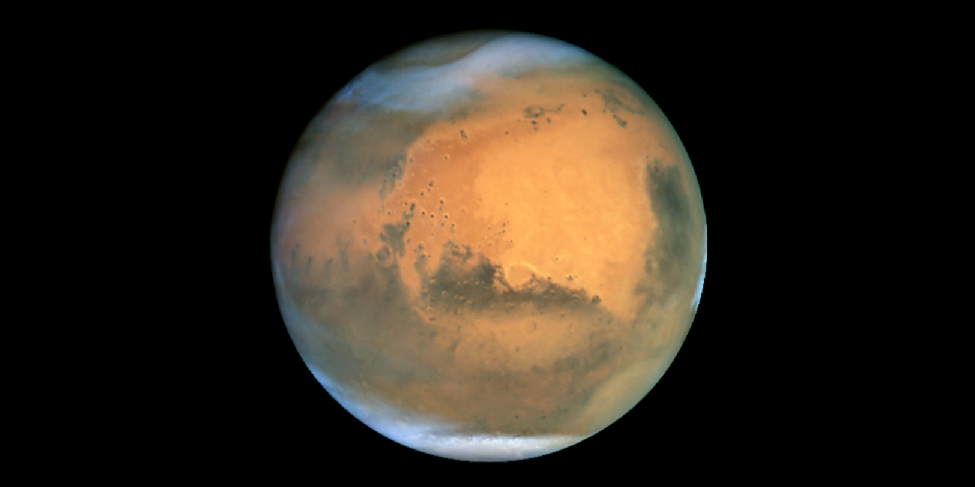
\includegraphics[width=6cm,trim={4cm 2mm 4cm 2mm}, clip]{Figures/Figure10.13.jpeg}};
    \end{tikzpicture}
    \captionsetup{margin=1in,type=figure,font=scriptsize}
    \captionof{figure}{\textbf{Mars Photographed by the Hubble Space Telescope}. This is one of the best photos of Mars taken from our planet, obtained in June 2001 when Mars was only 68 million kilometers away. (credit: modification of work by NASA and the Hubble Heritage Team (STScI/AURA))
}
\end{center}

For a few decades around the turn of the twentieth century, some astronomers believed that they saw evidence of an intelligent civilization on Mars. The controversy began in 1877, when Italian astronomer Giovanni Schiaparelli (1835--1910) announced that he could see long, faint, straight lines on Mars that he called \textit{canale}, or channels. In English-speaking countries, the term was mistakenly translated as ``canals,'' implying an artificial origin.

\vspace{1em}

Even before Schiaparelli's observations, astronomers had watched the bright polar caps change size with the seasons and had seen variations in the dark surface features. With a little imagination, it was not difficult to picture the canals as long fields of crops bordering irrigation ditches that brought water from the melting polar ice to the parched deserts of the red planet. (They assumed the polar caps were composed of water ice, which isn't exactly true, as we will see shortly.)

\vspace{1em}

Astronomers have determined the rotation period of Mars with great accuracy by watching the motion of permanent surface markings; its sidereal day is 24 hours 37 minutes 23 seconds, just a little longer than the rotation period of Earth. This high precision is not obtained by watching Mars for a single rotation, but by noting how many turns it makes over a long period of time. Good observations of Mars date back more than 200 years, a period during which tens of thousands of martian days have passed. As a result, the rotation period can be calculated to within a few hundredths of a second.

\vspace{1em}

The rotational axis of Mars has a tilt of about \ang{25}, similar to the tilt of Earth's axis \ang{23.5}. Thus, Mars experiences seasons very much like those on Earth. Because of the longer martian year (almost two Earth years), however, each season there lasts about six of our months.

\vspace{1em}

Mars is rather small, with a mass only 0.11 times the mass of Earth. However, it is larger than either the Moon or Mercury, and, unlike them, it retains a thin atmosphere. Mars is also large enough to have supported considerable geological activity in the distant past. But the most fascinating thing about Mars is that long ago it probably had a thick atmosphere and seas of liquid water---the conditions we associate with development of life. There is even a chance that some form of life persists today in protected environments below the martian surface.
			
\clearpage

Here are some basic properties of Mars, compared to Earth's.

\begin{center}
\begin{tabular}{|l|c|c|}
\hline
\textbf{Property} & \textbf{Earth} & \textbf{Mars}\\
\hline
Semimajor axis (AU)	& 1.00	& 1.52\\ \hline	
Period (days) & 365 & 687 \\	\hline	
Mass (Earth = 1) & 1.00 & 0.11 \\	\hline	
Diameter (km)	& \num{12756} & \num{6790}\\ \hline	
Density (\SI{}{g/cm^3})	& 5.5	&  3.9\\\hline	
Surface gravity (Earth = 1)	& 1.00	& 0.38\\	\hline	
Escape velocity (km/s)	& 11.2	& 5.0 \\	\hline	
Rotation period & 23.9 hours & 24.6 hours \\ \hline	
Surface area (Earth = 1) & 1.00 & 0.28 \\	\hline	
Atmospheric pressure (bar)	& 1.00 & 0.007\\ 
\hline
\end{tabular}
\end{center}

\subsection*{\ref{3uBag7} Exercises}

\begin{exercise}
    Why is Mars red?
\end{exercise}

\begin{exercise}
    Identify the average distance from the Sun to Mars, both in kilometers and in astronomical units.
\end{exercise}

\begin{exercise}
    Summarize the features of Mars that lead some people over 100 years ago to believe that there was an intelligent civilization living on Mars.
\end{exercise}

\begin{exercise}
    Recall that Venus takes a whopping 243 days to rotate once on its axis. What is Mars' rotation period?
\end{exercise}

\begin{exercise}
    Why does Mars have seasons, like the Earth?
\end{exercise}

\begin{exercise}
    On Earth, each of the four seasons lasts about 3 months. How long does a season last on Mars?
\end{exercise}

\begin{exercise}
    State the mass of Mars as a decimal fraction of Earth's mass. 
\end{exercise}

\begin{exercise}
    True or false? Mars lacks an atmosphere.
\end{exercise}

\begin{exercise}
    If microscopic life does exist on Mars today, where could it be found?
\end{exercise}

\begin{exercise}
    How many days does it take Mars to orbit the Sun one time? \textit{Hint}: This is known as the period.
\end{exercise}

\clearpage

\subsection*{Lesson Plans}

\begin{tabular}{|m{0.25\textwidth}|m{0.7\textwidth}|}
    \hline  
    \cellcolor{black!20}\textbf{Date} &
    \cellcolor{black!20}\textbf{Tuesday, April, 25 2023} \\
    \hline
    Learning Intention (TPO) & We will\ldots. \\
    \hline
    Hook/Warm Up/Opening & Students finish exercises from previous day.\\
    \hline
    Lesson/Learning Activities & Introduce Mars with brief PowerPoint presentation containing only images (no text). Summarize basic facts from \textit{Children's Atlas of the Universe} (p.~48), such as origin of name, distance from the sun, length of year, etc. Show Mars' two moons as seen through Stellarium. Show images of Mars' landscape. Presentation should be between 5--10 minutes tops.\\
    \hline
    Graded Activities & \\
    \hline
    Closure & \\  
    \hline
\end{tabular}








\end{document}

cycle list={
    only marks,mark=*,fill=gray,draw=black,mark size=1pt\\
    only marks,mark=*,fill=gray,draw=black,mark size=1pt\\
  },
  domain=270:360+90,
  samples=500,
  title={N=500,\dots},
  grid,
  axis equal
]

\addplot ({(0.5+0.07*rand)*cos(x)},{(0.5+0.07*rand)*sin(x)});
\addplot ({(1+0.1*rand)*cos(x)},{(1+0.1*rand)*sin(x)});